\documentclass[11pt,a4paper]{article}

\usepackage{datetime}
\usepackage{graphicx}
\usepackage{subcaption}

\usepackage{hyperref}

\hypersetup{
    colorlinks=true,
    linkcolor=blue,
    filecolor=magenta,      
    urlcolor=cyan,
}


\title{Chapter 4 Lab Work: Communication}
\newdate{date}{12}{05}{2020}
\date{\displaydate{date}}
\author{Nguyen Ngoc Lam - 20162316}

\begin{document}
	\pagenumbering{gobble}
  	\maketitle
  	\newpage
  	\tableofcontents
  	\newpage
  	
  	\section{What is the code part that shows that the Server assigns the correlation ID to the response?}
  	\begin{figure}[h!]
  		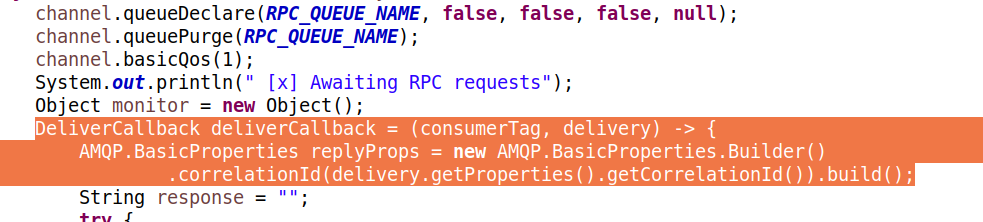
\includegraphics[width=\linewidth]{assign-corr-id.png}
  		\caption{Assigning correlation ID}
  		\label{fig:corr-id}
	\end{figure}
  	The part the Server assigns the correlation ID is highlighted in the figure \ref{fig:corr-id}
	
	\section{You base on both code of Client and Server program to explain which code shows that the Client sends request to Server through rpc\_queue and create a new queue to wait for the reply of the Server.}
	\begin{figure}[h!]
		\centering
  		\begin{subfigure}[b]{0.4\linewidth}
  		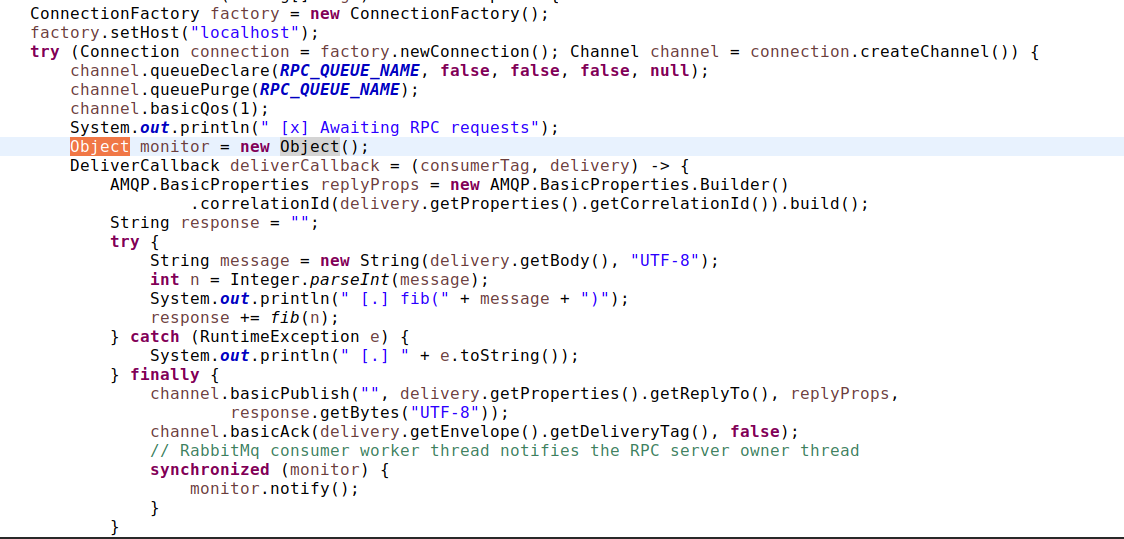
\includegraphics[width=\linewidth]{server-rpc-queue.png}
    		\caption{Receive request and response to request Server side}
  		\end{subfigure}
  		\begin{subfigure}[b]{0.4\linewidth}
    		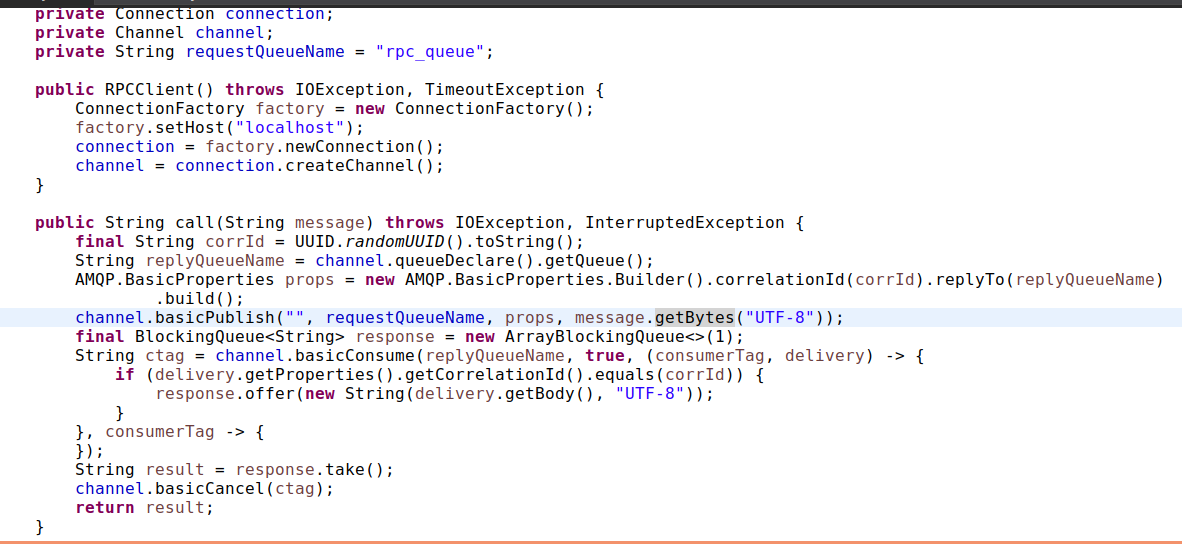
\includegraphics[width=\linewidth]{client-rpc-queue.png}
    		\caption{Sending request, create a new queue to wait the reply on Client side}
  		\end{subfigure}
  		\caption{Client sends request to Server through rpc\_queue}
  		\label{fig:rpc}
	\end{figure}
	
	\section{Try to add the delay to the Server program}
	The response from Server will be delayed thus making the Client waits for the response from previous request longer.\newpage
	\begin{figure}[t]
  		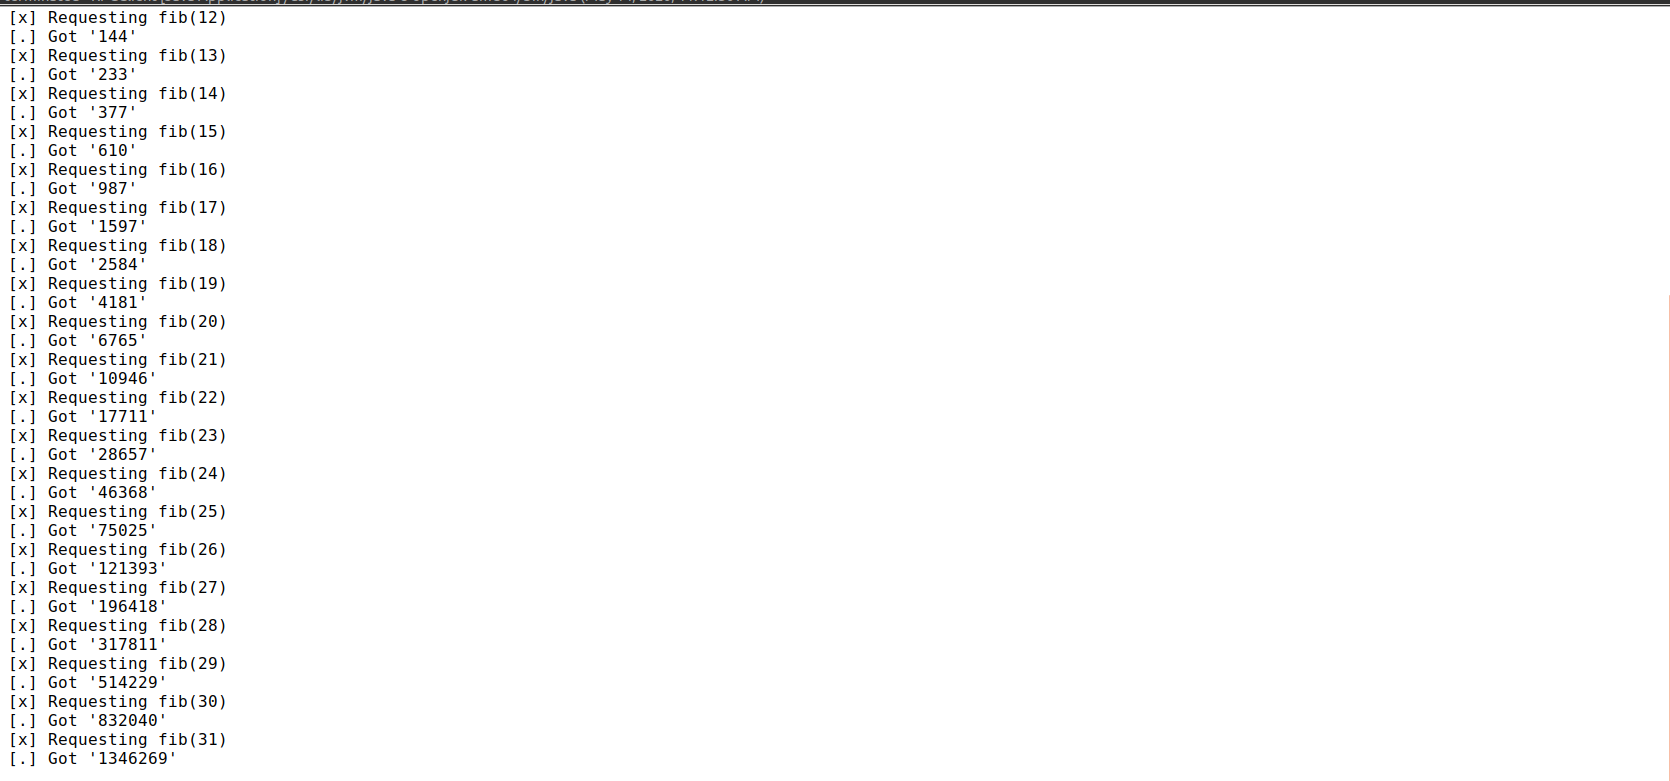
\includegraphics[width=\linewidth]{res-client.png}
  		\caption{Client Result}
  		\label{fig:res-client}
	\end{figure}
	When checking for queues, for n instances of Client are running, there are n queues for each instances plus the rpc\_queue. At all time, there are n-1 ready messages and 1 unacknowledged messages at rpc\_queue since the number on ArrayBlockingQueue equals to 1. The message on n unique queues for n instances will be transfered to rpc\_queue very fast thus it could be said that the ready messages and unacknowledged messages number equals to 0.
	\begin{figure}[h!]
		\centering
  		\begin{subfigure}[b]{0.4\linewidth}
  		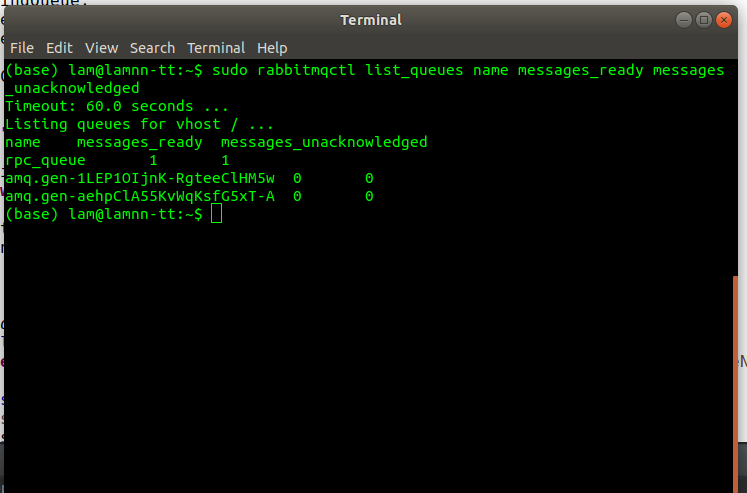
\includegraphics[width=\linewidth]{res-status.png}
    		\caption{When there are 2 instances of Client}
  		\end{subfigure}
  		\begin{subfigure}[b]{0.4\linewidth}
    		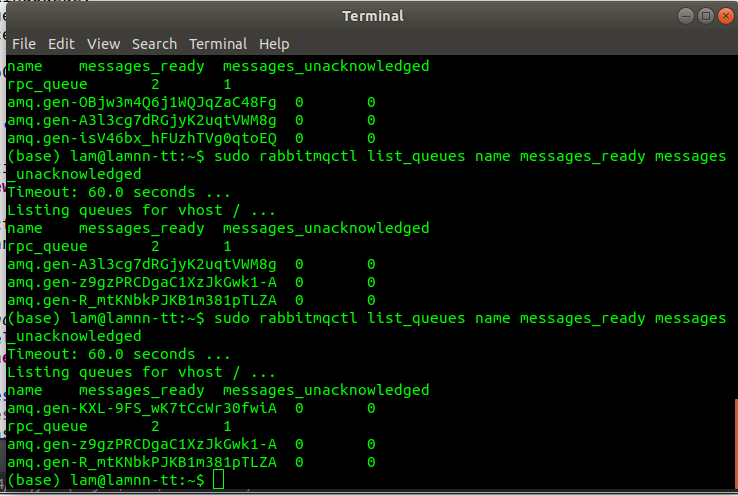
\includegraphics[width=\linewidth]{res-status-3.png}
    		\caption{When there are 3 instances of Client}
  		\end{subfigure}
  		\caption{Status of queues}
  		\label{fig:status}
	\end{figure}
	
	\section{Important note for the video streaming part.}
	\begin{enumerate}
		\item For this part, I will use my own laptop and my home computer connected over the home network.
	\end{enumerate}
	
	\section{What is the IP address of your 2 machines? How to ping each other?}
	The server will have the address: 192.168.0.109
	The client will have the address: 192.168.0.102
	\begin{figure}[h!]
		\centering
  		\begin{subfigure}[b]{0.4\linewidth}
  		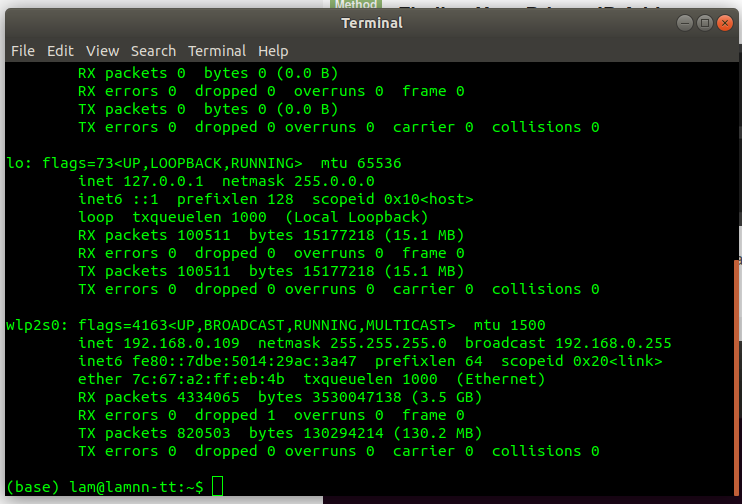
\includegraphics[width=\linewidth]{ip-server.png}
    		\caption{Of the Server}
  		\end{subfigure}
  		\begin{subfigure}[b]{0.4\linewidth}
    		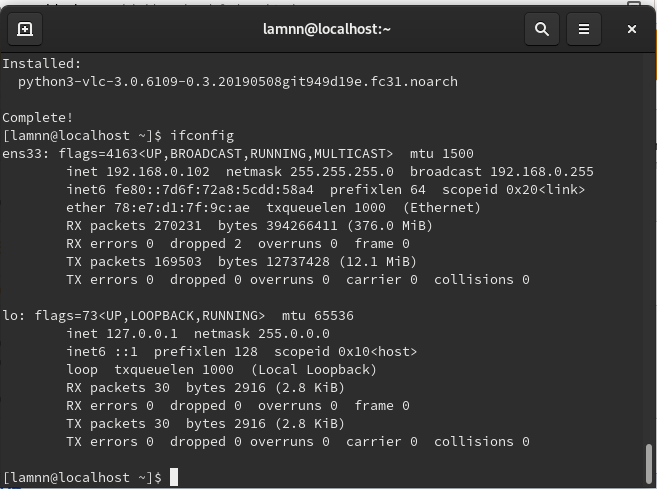
\includegraphics[width=\linewidth]{ip-client.png}
    		\caption{Of the Client}
  		\end{subfigure}
  		\caption{IP address}
  		\label{fig:addr}
	\end{figure}
	\\
	To ping each other we just use the standard ping function of Linux.
	\begin{figure}[h!]
  		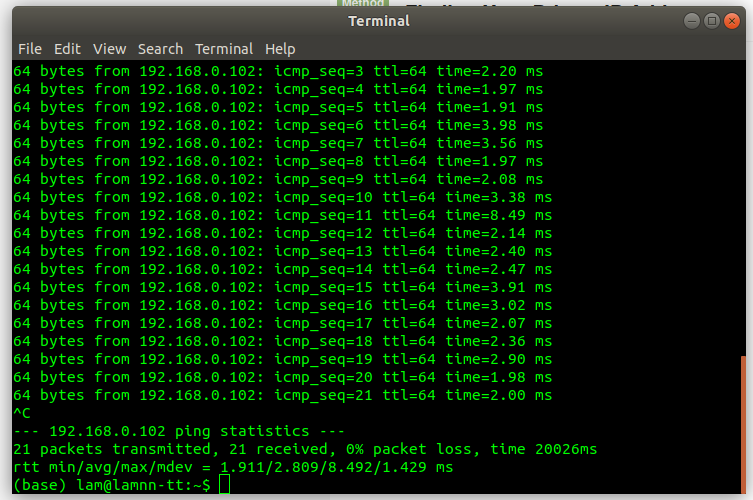
\includegraphics[width=\linewidth]{ping-to-client.png}
  		\caption{Ping from Server to Client}
  		\label{fig:ping}
	\end{figure}
	
	\section{Can you watch the video in the client machine? Evaluate the quality of the video streaming service.}
	When trying to connect to the server, we can see the video with good quality (no delay, no jitter, the stream is smooth)
	\begin{figure}[h!]
  		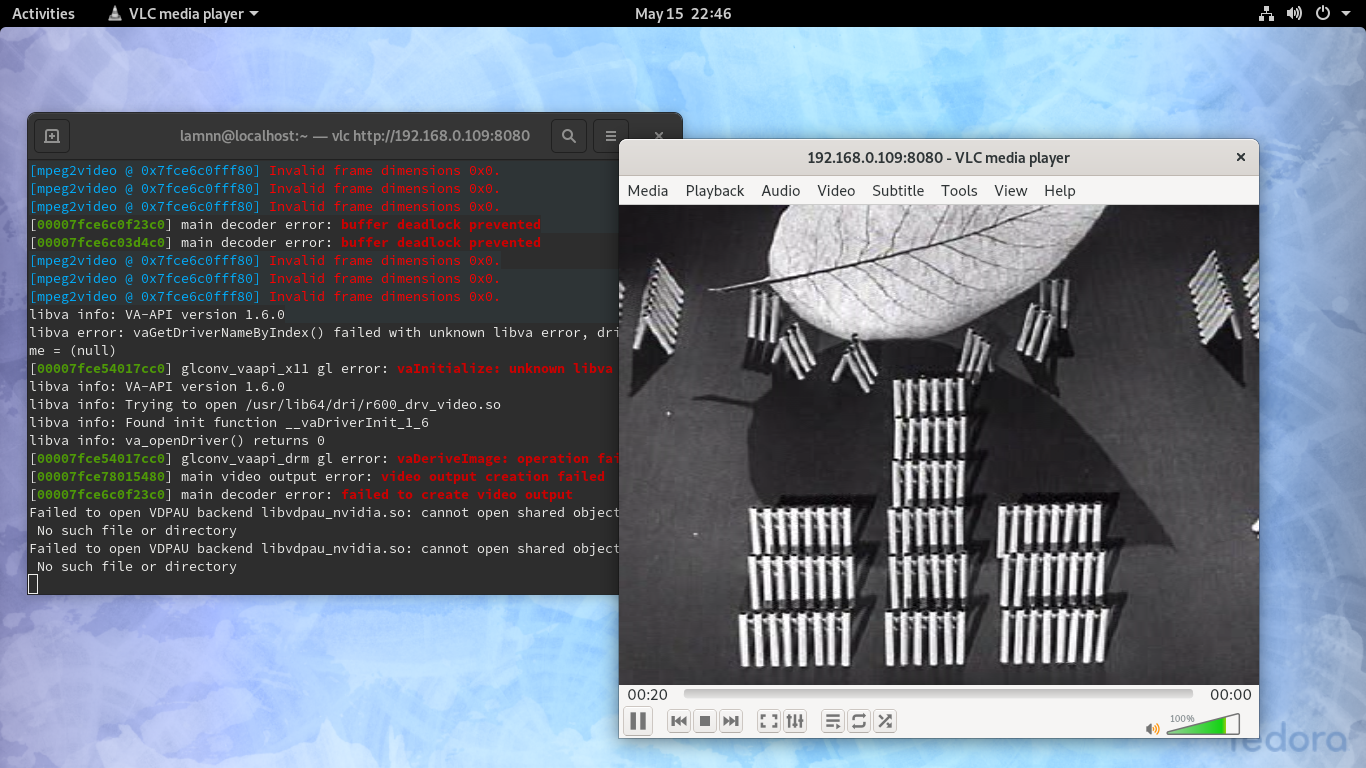
\includegraphics[width=\linewidth]{vid-perfect-cond.png}
  		\caption{Video streaming}
  		\label{fig:vid-p-cond}
	\end{figure}
	
	\section{What is the result of the ping test? Can you see an increase of 100 milliseconds?}
	\newpage
	\begin{figure}[h!]
  		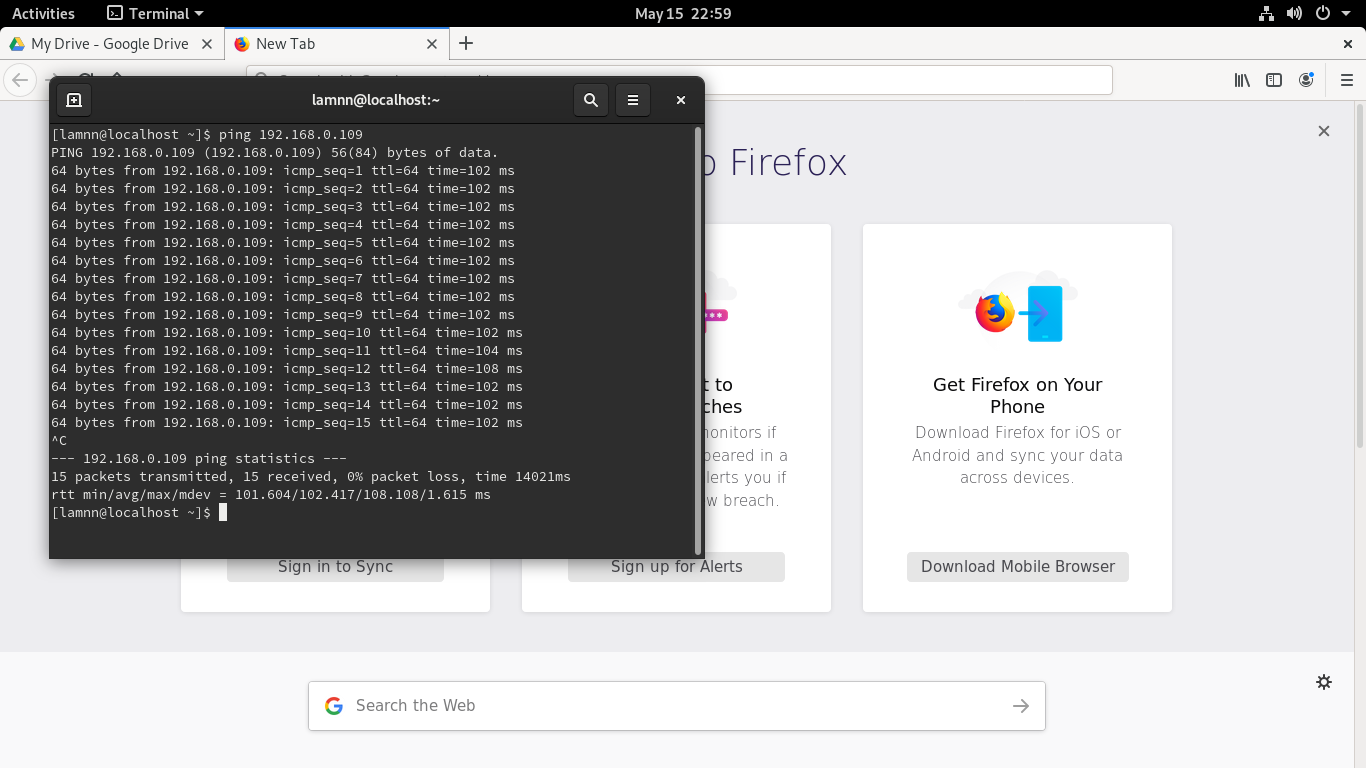
\includegraphics[width=\linewidth]{ping-delay-100.png}
  		\caption{Ping result when has delay=100ms}
  		\label{fig:ping-100}
	\end{figure}
	
	As figure \ref{fig:ping-100} shows, the time has been added 100ms from the previous time.
	
	\section{Disable the buffering function of VLC in Client machine. Then, evaluate the video quality at the Client machine. How can you conclude the impact of fix delay on video streaming service?}
	The frame periodically freezed. In conclusion, the impact of fix delay on video streaming service is constantly freeze the frames.
	
	\section{Evaluate the video quality atthe Client machine. How can you conclude the impact of delay variation on video streaming service?}
	The frame randomly freezed. In conclusion, the impact of delay variation on video streaming service is sometimes freeze the frames and for different duration.
	
	\section{Evaluate the video quality at the Client machine. How can you conclude the impact of fix loss rate on video streaming service? Try to increase the value of loss rate to see the impact more clear.}
	Sometimes, the video jumps from one scene to another scene without the transition. In conclusion, the impact of fix loss rate on video streaming service is the stream is periodically jitter. While it is annoying, if rate is low, it was bearable
	
	\section{Evaluate the video quality at the Client machine. How can you conclude the impact of loss rate variation on video streaming service? Try to increase this value to see the impact more clear.}
	There was a long duration of jitter. There was a 10 seconds black screen at some point.  In conclusion, the impact of loss rate variation on video streaming service is the stream is big gap in video. As a customer, this maybe unacceptable.
	
	\section{Evaluate the video quality at the Client machine. How can you conclude the impact of packet duplication on video streaming service? Try to increase this value to see the impact more clear.}
	There was a slight freeze at some frame.
	
	\section{Evaluate the video quality at the Client machine. How can you conclude the impact of packet corruption on video streaming service? }
	There is some frame that appeared after the frame that suppose to follow it. It makes the movement of the character seems to be backward.
\end{document}